%%%%%%%%%%%%%%%%%%%%%%%%%%%%%%%%%%%%%%%%%%%%%%%%%%%%%%%%%%%%%%%%%%
%%%%%%%%%%%%%%%%%%%%%%%%%%% ANNEXES	 %%%%%%%%%%%%%%%%%%%%%%%%%%%%%
%%%%%%%%%%%%%%%%%%%%%%%%%%%%%%%%%%%%%%%%%%%%%%%%%%%%%%%%%%%%%%%%%%

\appendix
\chapter{Lien vers les dépôts en ligne de la chaîne de traitement \ktb{}}
\chaptermark{Lien vers les dépôts}
L'intégralité du code produit pour le projet \ktb{}, depuis la création des documents \tei{} jusqu'à l'application Web, sont disponibles sur la plateforme d'hébergement de code GitHub.
\begin{itemize}
	\item \href{https://github.com/katabase}{Plateforme du projet}
	\item \href{https://github.com/katabase/1_OutputData}{Première étape: normalisation des documents \tei{}}
	\item \href{https://github.com/katabase/2_CleanedData}{Deuxième étape: extraction de données et normalisation}
	\item \href{https://github.com/katabase/3_WikidataEnrichment}{Troisième étape: enrichissement de données à l'aide de \wkd{}}
	\item \href{https://github.com/katabase/4_TaggedData}{Quatrième étape: création de jeux de données \json{} pour le site web}
	\item \href{https://github.com/katabase/Application}{Application web \ktb{}}
\end{itemize}

L'intégralité du code source est disponible sous licence libre (\href{https://www.gnu.org/licenses/gpl-3.0.html}{GNU GPL v3.0}, \href{https://mit-license.org/}{MIT} ou \href{https://creativecommons.org/}{Creative Commons}). Le site web peut également être consulté en ligne à \href{https://katabase.huma-num.fr/}{cette adresse}.

\chapter{Documentation des différentes étapes}
Ce chapitre contient la documentation des différentes étapes de la chaîne de traitement (en anglais), telle qu'elle se trouve sur les dépôts en ligne du projet sur GitHub. Cette documentation a simplement été convertie depuis le format \texttt{Markdown} vers \LaTeX{}.
\clearpage
\section*{Output Data - level 1}
\addcontentsline{toc}{section}{Output Data - level 1}

This repository contains digitised manuscripts sale catalogs encoded in XML-TEI at level 1.

The data have not been cleaned (\href{https://github.com/katabase/2\_CleanedData}{level 2}) or post-processed (\href{https://github.com/katabase/3\_TaggedData}{level 3}).
\section*{Description of the data}
\addcontentsline{toc}{subsection}{Description of the data}

Basic bibliographic information for each catalogue are available \href{https://github.com/katabase/1\_OutputData/blob/master/\_listDATA.csv}{here}.
\subsection*{Schema}
\addcontentsline{toc}{subsubsection}{Schema}

You can find the ODD that validates the encoding in the repository \href{https://github.com/katabase/Data\_extraction/tree/master/\_schemas}{Data\_extraction (folder \texttt{\_schemas})}.
\section*{Workflow}
\addcontentsline{toc}{subsection}{Workflow}
\subsection*{Creation of the data}
\addcontentsline{toc}{subsubsection}{Creation of the data}

The creation process is described in detail in the following \href{https://github.com/katabase/GROBID\_Dictionaries/blob/master/DOCUMENTATION.md}{repo}.
\subsection*{Cleaning the data}
\addcontentsline{toc}{subsubsection}{Cleaning the data}

Entries of catalogues look like the following:

\begin{listing}[h!]
   \begin{minted}{xml}
<item n="80" xml:id="CAT_000146_e80">
   <num>80</num>
   <name type="author">Cherubini (L.),</name>
   <trait>
   <p>l'illustre compositeur</p>
   </trait>
   <desc>L. a s.; 1836, 1 p 1 /2 in8.</desc>
   <measure commodity="currency" unit="FRF" quantity="12">12</measure>
</item>

   \end{minted}
\end{listing}

Most of the reconciliation process uses data from the \texttt{<desc\textgreater{}} element of our xml files. We therefore need to correct typos to ease further post-processing, \_e.g.\_
  * \texttt{L. a s.} -\textgreater{} \texttt{L. a. s.}
  * \texttt{in8} -\textgreater{} \texttt{in-8}
  * \texttt{1 /2} -\textgreater{} \texttt{1/2}
  * \texttt{1 p} -\textgreater{} \texttt{1 p.}

The \texttt{clean\_xml.py} script \href{https://github.com/katabase/1\_OutputData/blob/master/script/clean\_xml.py}{available here} tackles this problem.
\section*{Installation and use}
\addcontentsline{toc}{subsection}{Installation and use}

\begin{listing}[h!]
   \begin{minted}{bash}
* git clone https://github.com/katabase/1_OutputData.git
* cd 1_OutputData
* python3 -m venv my_env
* source my_env/bin/activate
* pip install -r requirements.txt
* python script/clean_xml.py -f FILENAME processes one single file
	OR
* python script/clean_xml.py -d DIRECTORY processes all the files contained in a directory

   \end{minted}
\end{listing}
\section*{Credits}
\addcontentsline{toc}{subsection}{Credits}

* The ODD was created by Lucie Rondeau du Noyer.

* \texttt{clean\_xml.py}was created by Simon Gabay.

* The catalogs were encoded by Lucie Rondeau du Noyer, Simon Gabay, Matthias Gille Levenson, Ljudmila Petkovic and Alexandre Bartz.

\section*{Cite this repository}
\addcontentsline{toc}{subsection}{Cite this repository}

Alexandre Bartz, Simon Gabay, Matthias Gille Levenson, Ljudmila Petkovic and Lucie Rondeau du Noyer, \_Manuscript sale catalogues\_, Neuchâtel: Université de Neuchâtel, 2019, \href{https://github.com/katabase/1\_OutputData}{https://github.com/katabase/1\_OutputData}.

\section*{Licence}
\addcontentsline{toc}{subsection}{Licence}

The catalogues are licensed under a \href{http://creativecommons.org/licenses/by/4.0/}{Creative Commons Attribution 4.0 International Licence} and the code is licensed under a GNU GPL-3.0 license.

\clearpage
\section*{Cleaned Data - level 2}
\addcontentsline{toc}{section}{Cleaned Data - level 2}

This repository contains digitised manuscripts sale catalogs encoded in XML-TEI at level 2.

The data have been cleaned (level 2) but not post-processed (\href{https://github.com/katabase/3\_TaggedData}{level 3}) yet.
\section*{Schema}
\addcontentsline{toc}{subsection}{Schema}

You can find the ODD that validates the encoding in the repository \href{https://github.com/katabase/Data\_extraction/tree/master/\_schemas}{Data\_extraction (folder \texttt{\_schemas})}.
\section*{Workflow}
\addcontentsline{toc}{subsection}{Workflow}

Once the data have been cleaned, we can start to extract information from the \texttt{desc}.

\texttt{extractor-xml.py} extracts informations and then retrieves them in the same XML file (level 3). 

The script transforms this

\begin{listing}[h!]
   \begin{minted}{xml}
<item n="80" xml:id="CAT_000146_e80">
   <num>80</num>
   <name type="author">Cherubini (L.),</name>
   <trait>
   <p>l'illustre compositeur</p>
   </trait>
   <desc>L. a. s.; 1836, 1 p. in-8.</desc>
   <measure commodity="currency" unit="FRF" quantity="12">12</measure>
</item>

   \end{minted}
\end{listing}

\pagebreak
into

\begin{listing}[h!]
   \begin{minted}{xml}
<item n="80" xml:id="CAT_000146_e80">
   <num>80</num>
   <name type="author">Cherubini (L.),</name>
   <trait>
   <p>l'illustre compositeur</p>
   </trait>
   <desc>
   <term>L. a. s.</term>;<date>1836</date>,
   	<measure type="length" unit="p" n="1">1 p.</measure> 
   	<measure unit="f" type="format" n="8">in-8</measure>.
   	<measure commodity="currency" unit="FRF" quantity="12">12</measure>
   </desc>
</item>

   \end{minted}
\end{listing}

To carry this task we use \texttt{extractor\_xml.py} \href{https://github.com/katabase/2\_CleanedData/tree/master/script/extractor-xml.py}{[available here}].
\section*{Installation and use}
\addcontentsline{toc}{subsection}{Installation and use}

\begin{listing}[h!]
   \begin{minted}{bash}
* git clone https://github.com/katabase/2_CleanedData.git
* cd 2_CleanedData
* python3 -m venv my_env
* source my_env/bin/activate
* pip install -r requirements.txt
* cd script 
* python3 extractor_xml.py directory_to_process

   \end{minted}
\end{listing}

\textbf{Note that you have to be in the folder \texttt{script}to execute \texttt{extractor\_xml.py} and that the script only works with filenames ending with \texttt{\_clean.xml} (files must have been beforehand cleaned).}

The output files will be in the folder \texttt{output}.
\section*{Credits}
\addcontentsline{toc}{subsection}{Credits}

* Scripts were created by Matthias Gille Levenson and improved by Alexandre Bartz with the help of Simon Gabay.
* The catalogs were encoded by Lucie Rondeau du Noyer, Simon Gabay, Matthias Gille Levenson, Ljudmila Petkovic and Alexandre Bartz.
\section*{Cite this repository}
\addcontentsline{toc}{subsection}{Cite this repository}

Alexandre Bartz, Simon Gabay, Matthias Gille Levenson, Ljudmila Petkovic and Lucie Rondeau du Noyer, \_Manuscript sale catalogues\_, Neuchâtel: Université de Neuchâtel, 2020, \href{https://github.com/katabase/2\_CleanedData}{https://github.com/katabase/2\_CleanedData}.
\section*{Licence}
\addcontentsline{toc}{subsection}{Licence}

The catalogues are licensed under a \href{http://creativecommons.org/licenses/by/4.0/}{Creative Commons Attribution 4.0 International Licence} and the code is licensed under a GNU GPL-3.0 license.

\clearpage
\section*{LEVEL 3 - WIKIDATA ENRICHMENTS}
\addcontentsline{toc}{section}{LEVEL 3 - WIKIDATA ENRICHMENTS}

\par\noindent\rule{\linewidth}{0.4pt}
\section*{Presentation}
\addcontentsline{toc}{subsection}{Presentation}

This part of the pipeline

\begin{itemize}
\item reconciles the names in our dataset with wikidata IDs
\item runs the same 4 \texttt{sparql} requests on all IDs
\item stores the output of the \texttt{sparql} requests in a \texttt{sparql} file
\item updates the \texttt{tei} files with the wikidata IDs 
\end{itemize}

The aim is to produce normlised data to connect to catalogue entries, in
order to understand our dataset better and to isolate the factors detrmining
a price.

\par\noindent\rule{\linewidth}{0.4pt}
\section*{Installation, pipeline and use}
\addcontentsline{toc}{subsection}{Installation, pipeline and use}

\par\noindent\rule{\linewidth}{0.4pt}
\subsection*{In short}
\addcontentsline{toc}{subsubsection}{In short}

With the proper python virtual environment sourced, without running tests, just type:

\begin{lstlisting}
shell
python main.py -n # build the input data table
python main.py -i # align tei:names with wikidata entities
python main.py -s # run sparql queries on those entities
python main.py -w # reinject the wikidata ids into the tei catalogues
\end{lstlisting}

Even simpler, you can just run the below script:

\begin{lstlisting}
shell
bash pipeline.sh
\end{lstlisting}

\par\noindent\rule{\linewidth}{0.4pt}
\subsection*{Installation}
\addcontentsline{toc}{subsubsection}{Installation}

This works on MacOS and Linux (ubuntu, debian based distributions).

\begin{lstlisting}
shell
git clone https://github.com/katabase/3_WikidataEnrichment # clone the repo
cd 3_WikidataEnrichment # move to the dictory
python3 -m venv env # create a python virtualenv
source env/bin/activate # source python from the virtualenv
pip install -r requirements.txt # install the necessary librairies
\end{lstlisting}

\par\noindent\rule{\linewidth}{0.4pt}
\subsection*{Pipeline and use}
\addcontentsline{toc}{subsubsection}{Pipeline and use}

All scripts run by running \texttt{main.py} with a specific argument. 4 GBs of RAM are recommended to
run the scripts. 

As a reminder, here is catalogue entries'\texttt{tei} 
structure:

\begin{listing}[h!]
   \begin{minted}{xml}
<item n="80" xml:id="CAT_000146_e80">
   <num>80</num>
   <name type="author">Cherubini (L.),</name>
   <trait>
   <p>l'illustre compositeur</p>
   </trait>
   <desc>
   <term>L. a. s.</term>;<date>1836</date>,
   <measure type="length" unit="p" n="1">1 p.</measure> 
   <measure unit="f" type="format" n="8">in-8</measure>.
   <measure commodity="currency" unit="FRF" quantity="12">12</measure>
   </desc>
</item>

   \end{minted}
\end{listing}

\par\noindent\rule{\linewidth}{0.4pt}

\textbf{Step 1 : create an input TSV} - \texttt{python main.py -n}

The first step is to create a \texttt{tsv} file that will be used to retrieve the wikidata IDs:

\begin{itemize}
\item the \texttt{tsv} is made of 5 columns (see example below):
\begin{itemize} 
 \item \texttt{xml id} : the item's \texttt{xml:id}
\item \texttt{wikidata id} : the wikidata ID (to be retrieved in the next step)
\item \texttt{name} : the \texttt{tei:name} of that item
\item \texttt{trait} : the \texttt{tei:trait} of that item 
\end{itemize}
\end{itemize}

\begin{table}[h]
\begin{tabular}{c|c|c|c}
xml id & wikidata id & name & trait \\
\hline 
CAT\_000362\_e27086 & & ADAM (Ad.) & célèbre compositeur de musique.
\end{tabular}
\end{table}


\begin{itemize}
\item \textbf{running this step}: 
\end{itemize}

\begin{lstlisting}
shell
python main.py -n
\end{lstlisting}

\par\noindent\rule{\linewidth}{0.4pt}

\textbf{Step 2 : retrieve the wikidata IDs} - \texttt{python main.py -i}

The wikidata IDs are retrieved by running a full text search using the 
\href{https://www.wikidata.org/w/api.php}{wikidata API}. 

\begin{itemize}
\item the \textbf{algorithm functions} as follows:
\begin{itemize} 
 \item the input is file created at the previous step (\texttt{script/tables/nametable\_in.tsv}). The \texttt{name} and \texttt{trait} columns are used to create data for the API search
\item two columns are processed to prepare the data for the API search:
\begin{itemize} 
 \item from the \texttt{name}, we determine the kind of \texttt{name} we're working with (the name of a person, of a nobility, of an event, of a place...). This determines different behaviours.
\item the \texttt{name} is normalized: we extract and translate nobility titles, locations... First and last names are extracted. If the first name is abbreviated, we try to rebuild a full name from its abbreviated version.
\item the \texttt{trait} is processed to extract and translate occupations, dates...
\item the output is stored in a dictionnary
\end{itemize}
\item this \texttt{dict} is passed to a second algorithm to run text searches on the API. Depending on the data stored in the dict, different queries are ran. A series of queries are run until a result is obtained
\item finally, the result is written to a TSV file (\texttt{out/wikidata/nametable\_out.tsv}). Its structure is the same as that of \texttt{nametable\_in}, with some changes. Here are the column names:
\begin{itemize} 
 \item \texttt{tei:xml\_id} : the \texttt{@xml:id} from the \texttt{tei} files
\item \texttt{wd:id} : the wikidata ID
\item \texttt{tei:name} : the \texttt{tei:name}
\item \texttt{wd:name} : the name corresponding to the wikidata ID (to ease the data verification process)
\item \texttt{wd:snippet} : a short summary of the wikidata page (to ease the data verification process)
\item \texttt{tei:trait} : the \texttt{tei:trait}
\item \texttt{wd:certitude} : an evaluation of the degree of certitude (whether we're certain that the proper id has been retrieved)
\end{itemize}
\item once this script has completed, a deduplicated list of wikidata IDs is written to \texttt{script/tables/id\_wikidata.txt}. This file will be used as input for the next step.
\item the F1 score for this step (evaluating the number of good wikidata IDs retrieved) is \texttt{0.674}, based on tests run on 200 items.
\item this step takes a lot of time to complete, but, thanks to log files, the script can be interrupted and restarted at any point.
\end{itemize}
\item \textbf{running this step} : 
\end{itemize}

\begin{lstlisting}
shell
python main.py -i
\end{lstlisting}

\par\noindent\rule{\linewidth}{0.4pt}

\textbf{Step 3 : running \texttt{sparql} queries} - \texttt{python main.py -s}

\begin{itemize}
\item the \textbf{algorithm} is much simpler: for each wikidata ID, 4 sparql queries are run. The results are returned in \texttt{json} or, if there's a mistake, \texttt{xml}. The results are translated to a simpler \texttt{json} and the result is stored to \texttt{out/wikidata/wikidata\_enrichments.json}. This step takes a lot of time, but the script can be stopped and continued at any point.
\item the \textbf{output structure} is as follows (each key is mapped to a list of results ; the list can be empty ; the empty lines in the dict separates the different wikidata queries): 
\end{itemize}

\clearpage
\begin{listing}[ph!]
   \begin{minted}{python}
   out = {'instance': [], 'instanceL': [], # what "category" an id belongs to (person, litterary work...)
   'gender': [], 'genderL': [], # the gender of a person
   'citizenship': [], 'citizenshipL': [], # citizenship
   'lang': [], 'langL': [], # languages spoken
   'deathmanner': [], 'deathmannerL': [], # the way a person died
   'birthplace': [], 'birthplaceL': [], # the place a person is born
   'deathplace': [], 'deathplaceL': [], # the place a person died
   'residplace': [], 'residplaceL': [], # the place a person lived
   'burialplace': [], 'burialplaceL': [], # where a person is buried

   'educ': [], 'educL': [], # where a person studied
   'religion': [], 'religionL': [], # a person's religion
   'occupation': [], 'occupationL': [], # general description of a person's occupation
   'award': [], 'awardL': [], # awards gained
   'position': [], 'positionL': [], # precise positions held by a person
   'member': [], 'memberL': [], # institution a person is member of
   'nobility': [], 'nobilityL': [], # nobility titles
   'workcount': [], # number of works (books...) documented on wikidata
   'conflictcount': [], # number of conflicts (wars...) a person has participated in
   'image': [], # url to the portrait of a person
   'signature': [], # url to the signature of a person
   'birth': [], 'death': [], # birth and death dates
   'title': [], # title of a work of art / book...
   'inception': [], # date a work was created or published
   'author': [], 'authorL': [], # author of a book
   'pub': [], 'pubL': [], # publisher of a work
   'pubplace': [], 'pubplaceL': [], # place a work was published
   'pubdate': [], # date a work was published
   'creator': [], 'creatorL': [], # creator of a work of art
   'material': [], 'materialL': [], # material in which a work of art is made
   'height': [], # height of a work of art
   'genre': [], 'genreL': [], # genre of a work or genre of works created by a person
   'movement': [], 'movementL': [], # movement in which a person or an artwork are inscribed
   'creaplace': [], 'creaplaceL': [], # place where a work was created
   'viafID': [], # viaf identifier
   'bnfID': [], # bibliothèque nationale de france ID
   'isniID': [], # isni id
   'congressID': [], # library of congress identifier
   'idrefID': [] # idref identifier}

   \end{minted}
\end{listing}

\begin{itemize}
\item \textbf{running this step}: 
\end{itemize}

\begin{lstlisting}
python main.py -s
\end{lstlisting}

\par\noindent\rule{\linewidth}{0.4pt}

\textbf{Step 4: reinject the wikidata ids into the TEI catalogues} - \texttt{python main.py -w}

\begin{itemize}
\item all \texttt{tei:items} are linked with a wikidata ID retrieved during the process. 
\item the wikidata IDs are included in a \texttt{@key} attribute inside the \texttt{tei:name} and prefixed by the token \texttt{wd:}.
\item a pattern to handle this prefix is provided in the \texttt{tei:teiHeader}, in the \texttt{tei:editorialDecl//tei:listPrefixDef}. this allows to automatically rebuilt a URL to the proper wikidata page.
\item the output is written to \texttt{out/catalogues}. 
\end{itemize}

\par\noindent\rule{\linewidth}{0.4pt}

\textbf{Running tests} - \texttt{python main.py -t}

\begin{itemize}
\item the tests are only run on the \textbf{step 2} (for the rest, we are certain of the result). 
\begin{itemize} 
 \item They are based on 200 catalogue entries. The test dataset ressembles the full dataset (about as many different kinds of entries, from different catalogues, with as many \texttt{tei:trait}s as in the main dataset)
\item Several tests are run. Two tests are testing isolate parameters of the dictionnary built in the step 1 and the efficiency of the function that rebuilds the first name from its abbreviation. The other tests are for the final algorithm and they build statistics it. They also calculate its execution time using different parameters.
\end{itemize}
\item \textbf{running the tests}: 
\end{itemize}

\begin{lstlisting}
python main.py -t
\end{lstlisting}

\par\noindent\rule{\linewidth}{0.4pt}

\textbf{Other options}:

\begin{itemize}
\item \textbf{counting the most used words in the \texttt{tei:trait}s} of the input dataset (to tweak the way the dictionnary is built in the step 2) : \texttt{python main.py -c}
\item \textbf{\texttt{python main.py -x}} : a throwaway option to map to a function in order to use a script that is not accessible from the above arguments 
\end{itemize}

\par\noindent\rule{\linewidth}{0.4pt}

\textbf{Summarizing, the options are}

\begin{lstlisting}
* -c --traitcounter : count most used terms in the tei:trait (to tweak the matching tables)
* -t --test : run tests (takes ~20 minutes)
* -i --wikidataids : retrieve wikidata ids (takes up to 10 to 20 hours!)
* -s --runsparql : run sparql queries (takes +-5 hours)
* -n --buildnametable: build the input table for -i --wikidataids (a table from which 
   to retrieve wikidata ids
* -x --throwaway : run the current throwaway script (to test a function or whatnot)
\end{lstlisting}

\par\noindent\rule{\linewidth}{0.4pt}
\section*{Credits}
\addcontentsline{toc}{subsection}{Credits}

Scripts developped by Paul Kervegan in spring-summer 2022. 

\par\noindent\rule{\linewidth}{0.4pt}
\section*{License}
\addcontentsline{toc}{subsection}{License}

The catalogues are licensed under a \href{http://creativecommons.org/licenses/by/4.0/}{Creative Commons Attribution 4.0 International Licence} and the code is licensed under a GNU GPL-3.0 license.

\clearpage
\section*{Tagged Data - level 3}
\addcontentsline{toc}{section}{Tagged Data - level 3}

This repository contains digitised manuscripts sale catalogs encoded in XML-TEI at level 3.

The data have been cleaned (\href{https://github.com/katabase/2\_CleanedData}{level 2}) and post-processed (level 3).
\section*{Schema}
\addcontentsline{toc}{subsection}{Schema}

You can find the ODD that validates the encoding in the repository \href{https://github.com/katabase/Data\_extraction/tree/master/\_schemas}{Data\_extraction (folder \texttt{\_schemas})}.
\section*{Workflow}
\addcontentsline{toc}{subsection}{Workflow}

Once the data have been cleaned and post-processed, we can check them. Some errors may appear and some corrections may be needed. 

From this data, \texttt{extractor-json.py} extracts informations and retrieves them in an JSON file, \href{https://github.com/katabase/3\_TaggedData/tree/main/output}{available here}.

The script transforms this 

\begin{listing}[h!]
   \begin{minted}{xml}
<item n="80" xml:id="CAT_000146_e80">
   <num>80</num>
   <name type="author">Cherubini (L.),</name>
   <trait>
   <p>l'illustre compositeur</p>
   </trait>
   <desc>
   <term>L. a. s.</term>;<date>1836</date>,
   <measure type="length" unit="p" n="1">1 p.</measure> 
   <measure unit="f" type="format" n="8">in-8</measure>.
   <measure commodity="currency" unit="FRF" quantity="12">12</measure>
   </desc>
</item>

   \end{minted}
\end{listing}

into 

\begin{listing}[h!]
   \begin{minted}{json}
{"CAT_000146_e80_d1": {"desc": "L. a. s.; 1836, 1 p. in-8. 12",
   "price": 12.0,
   "author": "Cherubini",
   "date": "1836",
   "number_of_pages": 1.0,
   "format": 8,
   "term": 7,
   "sell_date": "1893-03"}}

   \end{minted}
\end{listing}

From \texttt{export.json}, we can proceed at the reconciliation of the catalogues entries. 

If you want to learn more about the reconciliation, visite \href{https://raw.github.com/katabase/reconciliation}{this repository}. 

If you want to query the database, don't hesitate to try our \href{https://raw.github.com/katabase/application}{application}.
\section*{Installation and use}
\addcontentsline{toc}{subsection}{Installation and use}

\begin{listing}[h!]
   \begin{minted}{bash}
* git clone https://github.com/katabase/3_TaggedData.git
* cd 3_TaggedData
* python3 -m venv my_env
* source my_env/bin/activate
* pip install -r requirements.txt
* cd script 
* python3 extractor_json.py

   \end{minted}
\end{listing}
\textbf{Note that you have to be in the folder \texttt{script}to execute \texttt{extractor\_json.py}.}

The output file, \texttt{export.json}, is in the folder \texttt{output}.
\subsection*{Unittest}
\addcontentsline{toc}{subsubsection}{Unittest}

If you want run some unittests, try in the folder \texttt{script}: 

\begin{listing}[h!]
   \begin{minted}{bash}
python3 test.py

   \end{minted}
\end{listing}
\section*{Credits}
\addcontentsline{toc}{subsection}{Credits}

* The script was created by Alexandre Bartz with the help of Matthias Gille Levenson and Simon Gabay.
* The catalogs were encoded by Lucie Rondeau du Noyer, Simon Gabay, Matthias Gille Levenson, Ljudmila Petkovic and Alexandre Bartz.
\section*{Cite this repository}
\addcontentsline{toc}{subsection}{Cite this repository}

Alexandre Bartz, Simon Gabay, Matthias Gille Levenson, Ljudmila Petkovic and Lucie Rondeau du Noyer, \_Manuscript sale catalogues\_, Neuchâtel: Université de Neuchâtel, 2020, \href{https://github.com/katabase/3\_TaggedData}{https://github.com/katabase/3\_TaggedData}.
\section*{Licence}
\addcontentsline{toc}{subsection}{Licence}

The catalogues are licensed under a \href{http://creativecommons.org/licenses/by/4.0/}{Creative Commons Attribution 4.0 International Licence} and the code is licensed under a GNU GPL-3.0 license.
\clearpage
\section*{Application}
\addcontentsline{toc}{section}{Application}

This repository contains the web publication application of the corpus of manuscript 
sales catalogues. This branch contains the current stable version of the website. See
\texttt{versionX.X.X} for the older versions.

\par\noindent\rule{\linewidth}{0.4pt}
\section*{Getting started :}
\addcontentsline{toc}{subsection}{Getting started :}

\begin{itemize}
\item First, download this repository. Using command lines, clone the repository with : 
\end{itemize}

\begin{listing}[h!]
   \begin{minted}{bash}
git clone https://github.com/katabase/Application.git
cd Application

   \end{minted}
\end{listing}

\begin{itemize}
\item Then, create a virtual environment and activate it : 
\end{itemize}

\begin{listing}[h!]
   \begin{minted}{bash}
python3 -m venv my_env
source my_env/bin/activate

   \end{minted}
\end{listing}

\begin{itemize}
\item Now, you have to install dependencies : 
\end{itemize}

\begin{listing}[h!]
   \begin{minted}{bash}
pip install -r requirements.txt

   \end{minted}
\end{listing}

\begin{itemize}
\item You can finally launch the application : 
\end{itemize}

\begin{listing}[h!]
   \begin{minted}{bash}
python3 run.py

   \end{minted}
\end{listing}

\par\noindent\rule{\linewidth}{0.4pt}
\section*{Use the \texttt{KatAPI}}
\addcontentsline{toc}{subsection}{Use the \texttt{KatAPI}}

\texttt{KatAPI} is an API that allows the automated retrieval of data from the project in 
\texttt{json} or \texttt{xml-tei}. The API allows to revtrieve catalogue entries by author, sale date
and original date of the manuscript; it also allows to retrieve a complete catalogue, or
statistics on one or several catalogues. Finally, it creates custom error messages in \texttt{json}
of \texttt{tei} if an error occurs. For a more complete description, please see the Katabase website.
\subsection*{Quick start}
\addcontentsline{toc}{subsubsection}{Quick start}

The endpoint for the API is \textbf{\texttt{https://katabase.huma-num.fr/katapi?}}. The arguments 
provided by the client are added after this endpoint; the application will process
thoses arguments and send back a response in the requested format (\texttt{json} or \texttt{xml-tei},
the default being \texttt{json}). If there is an error on the client side (unauthorized 
parameters or values) or on the server side (unexpected error), a response will be
issued in \texttt{json} or \texttt{xml-tei} (depending on the client's request) describing the 
query parameters, the time of the query and the error that occured.
\subsection*{Possible query parameters and authorized values}
\addcontentsline{toc}{subsubsection}{Possible query parameters and authorized values}

\noindent{}\textbf{HTTP methods}

The only \textbf{authorized HTTP method} is \texttt{GET}.

\noindent{}\textbf{Possible parameters}

The \textbf{possible parameters} are:

\begin{itemize}
\item \textbf{\texttt{format}}: the format of the API's response body. Possible values are:
\begin{itemize} 
 \item \texttt{json}: \textbf{this is the default value}.
\item \texttt{tei}: return an \texttt{xml-tei} response.
\end{itemize}
\item \textbf{\texttt{level}}: the requested data's level. Possible values are:
\begin{itemize} 
 \item \texttt{item}: data is retrieved at item level. \textbf{This is the default value.}
\item \texttt{cat\_data}: statistical data on one or several catalogues will be retrieved
\begin{itemize} 
 \item this value is incompatible with the \texttt{orig\_date} parameter.
\end{itemize}
\item \texttt{cat\_full}: a complete catalogue encoded in \texttt{xml-tei} will be retrieved
\begin{itemize} 
 \item if this value is provided, then the only other authorized parameters are 		 \texttt{format=tei} and \texttt{id} (with \texttt{id} matching \texttt{CAT-\textbackslash{}d+}).
\end{itemize}
\end{itemize}
\item \textbf{\texttt{id}}: the identifier of the item or catalogue(s) to retrieve (depending on the value of \texttt{level}). If this parameter is provided, data will only be retrieved for a single catalogue or catalogue entry. This parameter cannot be used together with the \texttt{name} parameter. Possible values are:
\begin{itemize} 
 \item if the query is at item level, a catalogue entry's \texttt{@xml:id}. This identifier 	 is a string that matches the pattern: \texttt{CAT\_\textbackslash{}d+\_e\textbackslash{}d+\_d\textbackslash{}d+}.
\item the query is run at catalogue level (\texttt{level=cat\_full} or \texttt{level=cat\_data}), a 	 catalogue's \texttt{@xml:id}. This identifier is a string that matches the pattern: 	 \texttt{CAT\_\textbackslash{}d+}.
\end{itemize}
\item \textbf{\texttt{name}}: if the \texttt{id} parameter is not supplied, the name of the catalogue(s) or catalogue entry(ies) to retrieve. Note that this parameter can, and will, return several items. Possible values:
\begin{itemize} 
 \item if \texttt{level=item}, the \texttt{tei:name} being queried. Only the last name in 	 the \texttt{tei:name} is indexed in the search engine and only this one will yield a 	 result. If a first name and a last name are provided, no result can be yield, since the first name is not indexed.
\item if \texttt{level=cat\_stat}, the catalogue type (to be found in 	 \texttt{(TEI//sourceDesc/bibl/@ana} in the \texttt{xml} representation of a catalogue). 	 Possible values are:
\begin{itemize} 
 \item ``LAC": Vente Jacques Charavay,
\item ``RDA": Revue des Autographes,
\item ``LAV": Catalogue Laveredet,
\item ``AUC": Auction sale
\item ``OTH": not yet in use in our dataset
\end{itemize}
\end{itemize}
\item \textbf{\texttt{sell\_date}}: the sale date for a manuscript or a catalogue. Values must match the regular expression \texttt{\textbackslash{}d\{4\}(-\textbackslash{}d\{4\})?}: a year in \texttt{YYYY} format or a year range in \texttt{YYYY-YYYY} foramat.
\item \textbf{\texttt{orig\_date}}: the date a manuscript item was created. This parameter is only authorized if \texttt{level=item}. Values must match the regular expression \texttt{\textbackslash{}d\{4\}(-\textbackslash{}d\{4\})?}: a year in \texttt{YYYY} format or a year range in \texttt{YYYY-YYYY} foramat. 
\end{itemize}

\pagebreak
\par\noindent\rule{\linewidth}{0.4pt}
\section*{Workflow}
\addcontentsline{toc}{subsection}{Workflow}
\begin{figure}[h]
	\centering
	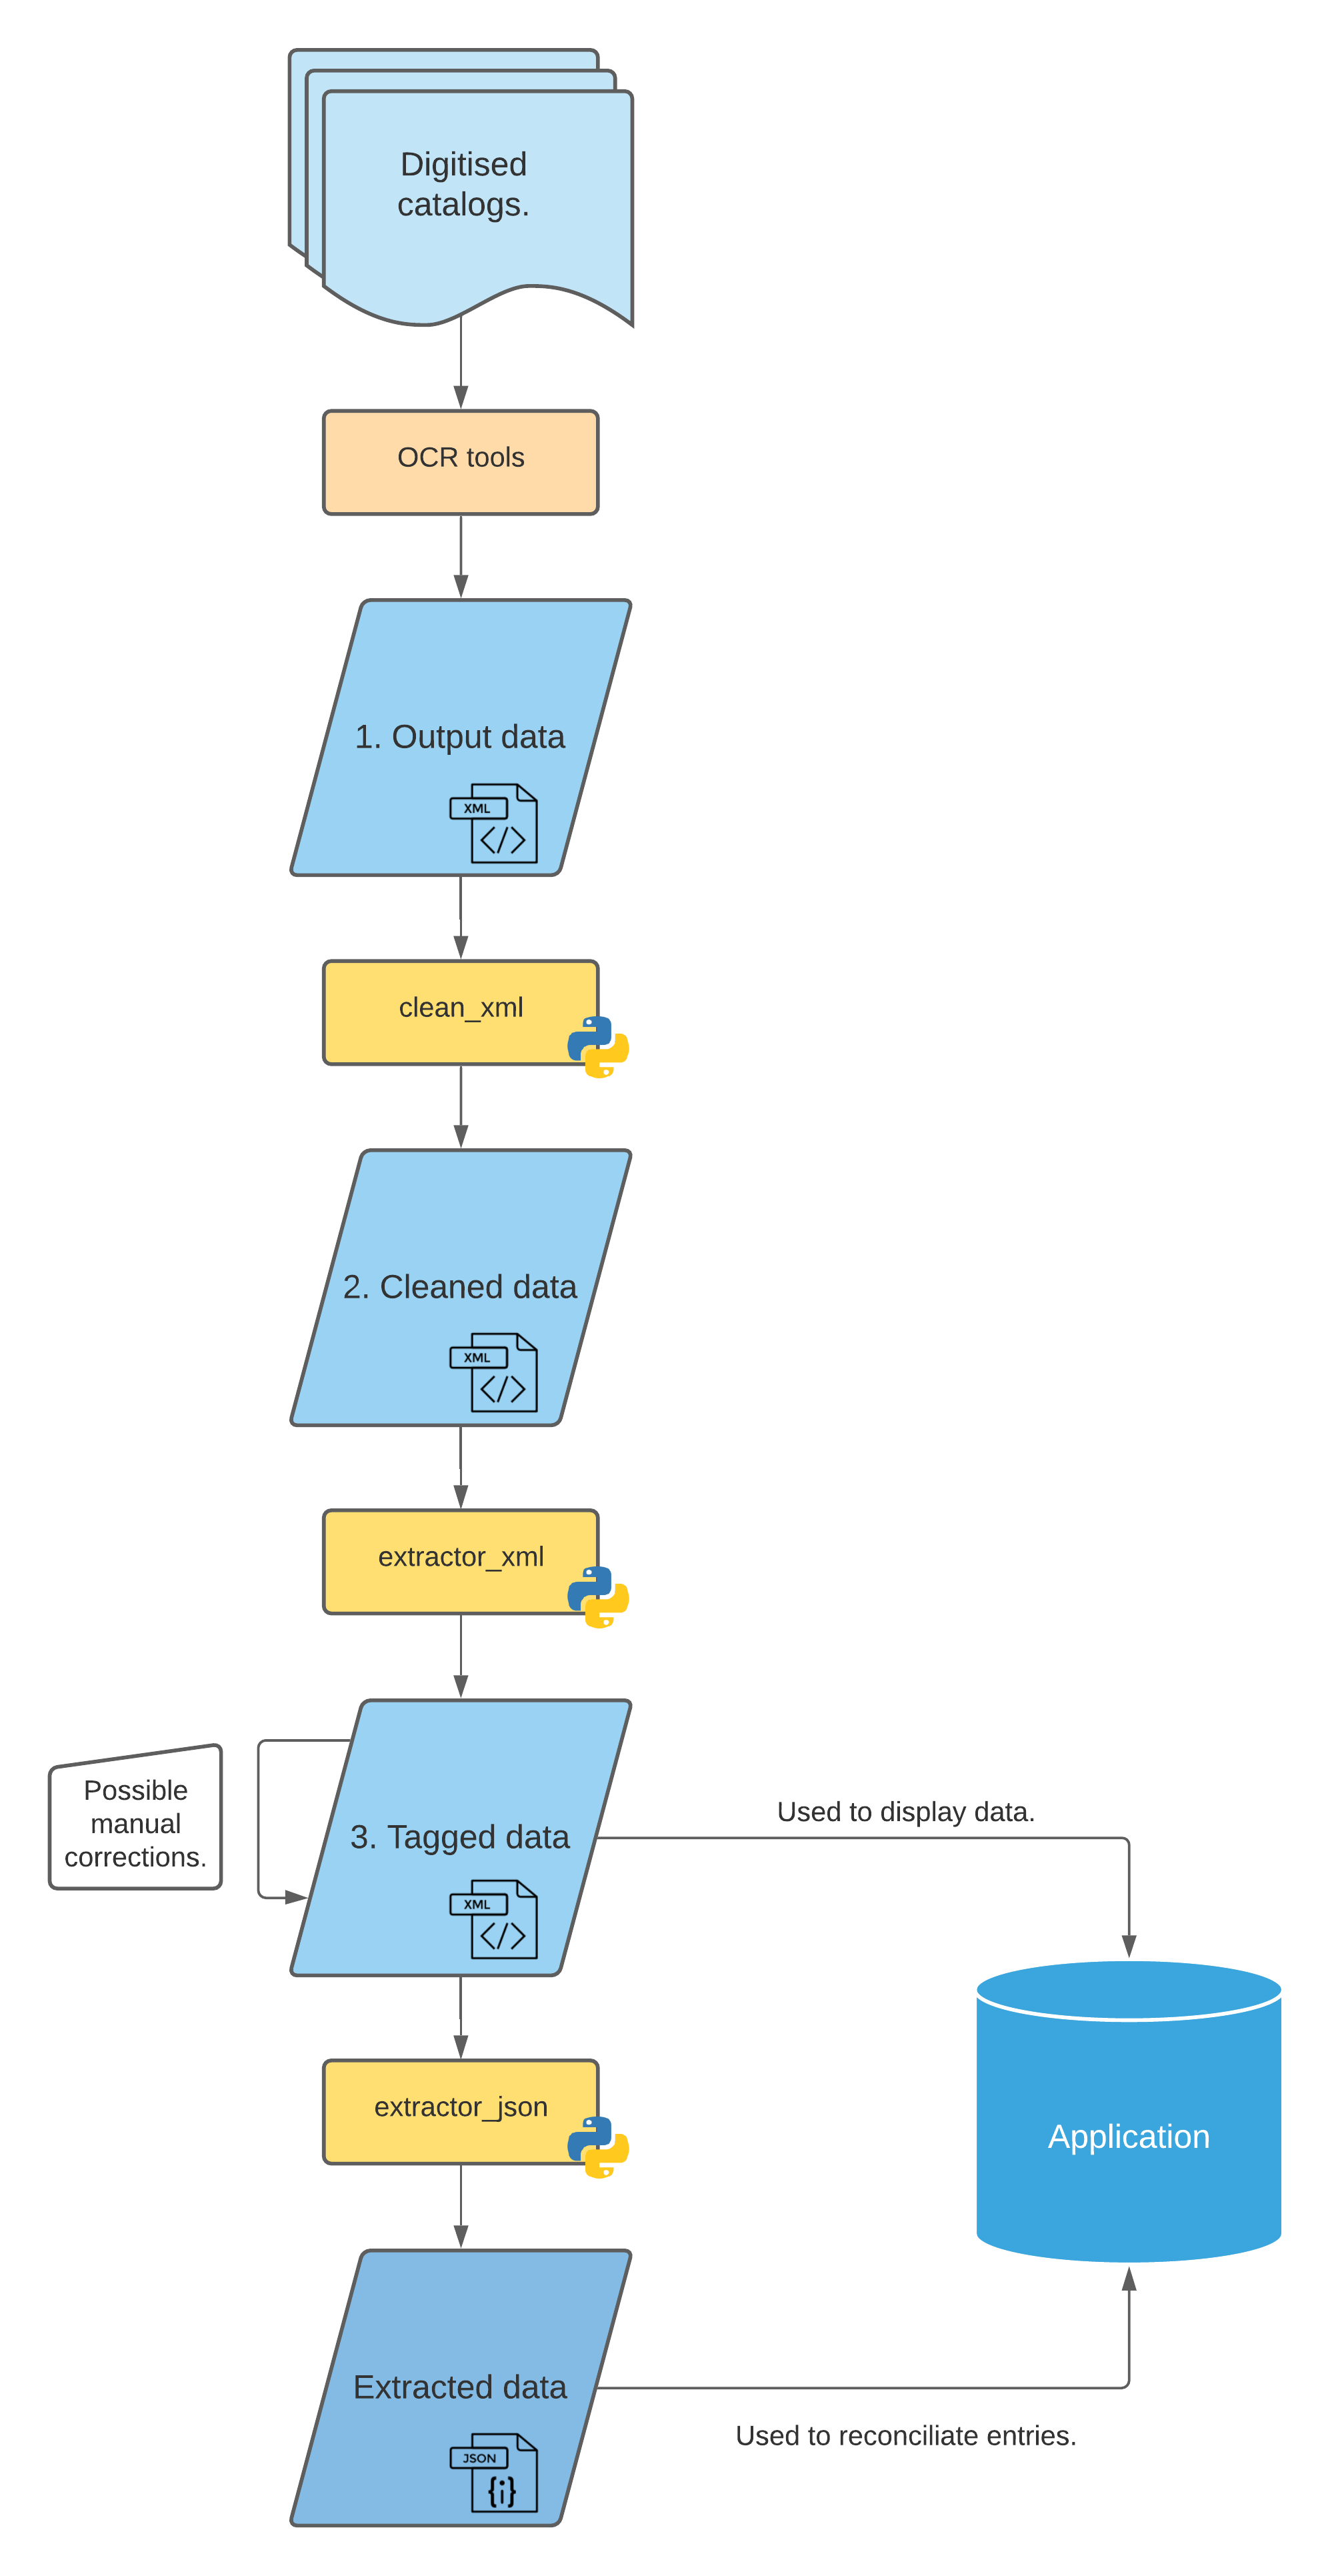
\includegraphics[height=\textwidth]{./annexes/workflow.png}
\end{figure}

\par\noindent\rule{\linewidth}{0.4pt}
\section*{Website updates and description of the git branches}
\addcontentsline{toc}{subsection}{Website updates and description of the git branches}

The structure of the git repository is as follows:

\begin{itemize}
\item \href{https://github.com/katabase/Application}{\texttt{main}} for the current, stable version of the Katabase app
\item \href{https://github.com/katabase/Application/tree/dev}{\texttt{dev}} for the unstable version of the app, in developpment and not running online.
\item \href{https://github.com/katabase/Application/tree/version1.0.0}{\texttt{versionX.X.X}} are archive repositories to document the former versions of the Katabase app. There should be as many of these branches as there are new versions of the website, and their \texttt{X.X.X} code should follow the release numbers. 
\end{itemize}

New additions to the website should be done on \texttt{dev} and tested before being moved to \texttt{main}.
The version of the website visible on \texttt{main} should be the same as the version of the website
online (unless, for reasons out of our control, we can't publish a new version of the website
online, but a new version is ready and won't be changed again). Before merging a new version
of the website from \texttt{dev} to \texttt{main}, the \texttt{main} branch should be moved the \texttt{versionX.X.X}.
A new release should then be created for the updated version of the website.

\par\noindent\rule{\linewidth}{0.4pt}
\section*{Credits}
\addcontentsline{toc}{subsection}{Credits}

The application was designed by Alexandre Bartz and Paul Kervegan with the help of Simon Gabay, Matthias Gille Levenson and Ljudmila Petkovic.

\par\noindent\rule{\linewidth}{0.4pt}
\section*{Cite this repository}
\addcontentsline{toc}{subsection}{Cite this repository}

\section*{Licence}
\addcontentsline{toc}{subsection}{Licence}

The catalogues are licensed under a \href{http://creativecommons.org/licenses/by/4.0/}{Creative Commons Attribution 4.0 International Licence} and the code is licensed under a GNU GPL-3.0 license.


\chapter{Résultat des tests de l'algorithme d'extraction d'informations de \wkd{}}
\chaptermark{Résultat des tests}

Les résultats des tests présentés dans les tables ci-dessous (\ref{appendix:testisolate}, \ref{appendix:testfinal}) ont été menés sur un jeu de 200 couples \tname{} et \ttrait{}. Ils ont été choisis de façon à être représentatifs du jeu de données complet, avec une variété d'entrées semblables (personnes nobles et non nobles, entrées qui ne sont pas consacrées à des personnes...). Ce jeu de test présente également une structure et un degré de détail semblable au jeu de données complet. Il y a notamment exactement la même proportion d'entrées présentant un \ttrait{} que dans le jeu de test et le jeu final.

Les résultats en pourcentage sont toujours exprimés en \textbf{pourcentages du nombre total d'entrées requêtées} (soit 200).
\pagebreak

\begin{table}[h]
	\centering
	\begin{tabular}{>{\centering}m{3cm}m{2cm}m{2cm}m{2cm}m{2cm}m{2cm}}
		\hline
		\textbf{Type de requête} & \textbf{Noms} & \textbf{Noms et nom de famille noble} & \textbf{Noms et titre de noblesse} & \textbf{Noms et date de naissance et de mort} & \textbf{Noms et occupation} \\
		\hline
		\hline
		Avec reconstitution des prénoms & 48\% & 45.9\% & 50\% & 52.6\% & 53.1\% \\
		\hline
		Sans reconstitution des prénoms & 42\% & 40.5\% & 50\% & 52.6\% & 53.1\% \\
		\hline	
	\end{tabular}
	\caption{Tests menés avec un jeu de 200 entrées sur des paramètres isolés}
	\label{appendix:testisolate}
\end{table}

Le tableau ci-dessus (\ref{appendix:testisolate}) présente les résultats de tests menés pour isoler l'impact de chaque paramètee dans l'obtention du bon résultat. Les mêmes requêtes ont été lancées sur un jeu de test de 200 entrées de catalogue. Toutes les requêtes contient le prénom et le nom de famille complets (\enquote{Noms} dans la table). La première requête ne contient que ce paramètre, tandis que toutes les autres requêtes sont lancées avec un paramètre en plus: titre de noblesse, nom de famille noble, dates et occupation. Le fait que ces paramètres soient utilisés ne garantit pas qu'ils soient disponibles dans le jeu de données utilisé en entrée.  Ce test permet d'isoler de mieux construire l'algorithme final de recherches en plein texte sur le moteur de recherche de \wkd{}, puisqu'il permet de voir quels sont les paramètres les plus fiables.
\vfill
\clearpage


\begin{table}[h]
	\centering
	\begin{tabular}{m{10cm}m{4cm}}
		\textbf{Bons identifiants récupérés} & 65\% \\
		\hline
		\textbf{Score F1 } & 0.674 \\
		\hline
		\textbf{Précision } & 0.677 \\
		\hline
		\textbf{Rappel } & 0.670 \\
		\hline
		\textbf{Résultats certains } & 36\% \\
		\hline
		\textbf{Faux positifs parmi les éléments certains} & 8.5\% \\
		\hline
		\textbf{Total d'entrées requêtées } & 200 \\
		\hline
		\textbf{Identifiants récupérés } & 192 \\
		\hline
		\textbf{Silence } & 8 \\
		\hline
		\textbf{Temps d'exécution avec l'option \texttt{fetch} } & 88.3 secondes \\
		\hline
		\textbf{Temps d'exécution sans l'option \texttt{fetch}} & 92.49 secondes \\
	\end{tabular}
	\caption{Tests menés avec un jeu de 200 entrées sur l'algorithme final}
	\label{appendix:testfinal}
\end{table}

Le tableau ci-dessus présente les résultats d'un test évaluant les performances de l'algorithme final. Voici une explication de ces résultats:
\begin{itemize}
	\item \textit{Bons identifiants récupérés}: la proportion, exprimée en pourcentage, du nombre d'identifiants récupérés par l'algorithme qui correspondent aux identifiants récupérés manuellement
	\item \textit{Score F1}: le \gls{score F1}, soit la moyenne pondérée de la précision et du rappel. Contrairement  à la mesure ci-dessus, le score F1 prend en compte le silence et les faux négatifs, et offre donc une interprétation plus complète de la qualité du script.
	\item \textit{Précision}: la précision est une composante du \gls{score F1} qui mesure la proportion d'identifiants pertinents obtenus parmi tous les identifiants obtenus.
	\item \textit{Rappel}: le rappel est une composante du \gls{score F1} qui mesure la proportion d'identifiants pertinents obtenus parmi l'ensemble des identifiants pertinents qui existent.
	\item \textit{Résultats certains}: pour accélérer le processus de relecture, un score de certitude a été attribué à certains identifiants obtenus grâce à l'algorithme. Ce score dépend du nombre de paramètres utilisés dans la recherche qui a permis de récupérer l'identifiant. 36\% des résultats obtenus sont considérés comme certains.
	\item \textit{Faux positifs parmi les éléments certains}: le score de certitude présenté ci-dessus admet un taux d'erreur qui est ici quantifié: 8.5\% des résultats obtenus sont erronnés alors qu'ils ont été considérés comme certains (8,5\% du jeu de données total, donc).
	\item \textit{Total d'entrées requêtées}: le volume du jeu de données de test, soit 200 entrées.
	\item \textit{Identifiants récupérés}: le nombre d'identifiants obtenus, qu'ils soient corrects ou non.
	\item \textit{Silence}: le nombre d'entrées pour lesquelles aucun identifiant n'a été obtenu.
	\item \textit{Temps d'exécution avec l'option \texttt{fetch}}: le temps pris, en secondes, pour lancer l'intégralité de l'algorithme de récupération d'identifiants \wkd{} sur les 200 entrées en stockant dans des \glspl{log} les requêtes lancées et les identifiants requêtés.
	\item \textit{Temps d'exécution sans l'option \texttt{fetch}}: le temps pris, en secondes, pour lancer l'intégralité de l'algorithme de récupération d'identifiants sur les 200 entrées sans utiliser de fichiers de log.
\end{itemize}
\clearpage

\begin{table}[h]
	\centering
	\begin{tabular}{m{5cm}m{3cm}m{3cm}m{3cm}}
		\diagbox[innerwidth=5cm]{Score}{Base de con-\\naissances} & Score F1 -- recherche des candidates & Score F1 -- Lien avec le candidat & Overall linking accuracy \\
		DBPedia & 0.899 & 0.536 & 0.834 \\
		DataBNF & 0.689 & 0.726 & 0.7 \\
		Wikidata & 0.869 & 0.611 & 0.85 \\
	\end{tabular}
	\caption{Résultats du \gls{nel} de lieux dans des textes littéraires du XIXe~s. par Soudani et al. (2018)}
	\label{appendix:soudani}
\end{table}
Scores obtenus par Aicha Soudani et al. pour le liage d'entités nommées pour des lieux dans des textes littéraires français du \scl{XIX}, présentés à la conférence \textit{HumaNS’2018}\footcite[p. 4]{soudani_adaptation_2018}. Les scores F1 ne figurent pas dans l'article original, qui ne présente que la précision et le rappel. Je les ai donc calculés moi même. La méthode de calcul de l'\textit{overall linking accuracy} (\enquote{exactitude générale du liage}) n'est pas précisée dans l'article; il est seulement indiqué que \enquote{Cette mesure essaie d'évaluer l'efficacité globale du système, et non par phase, et exprime la fiabilité de REDEN pour la tâche de résolution des entités nommées.}\footcite[p. 4]{soudani_adaptation_2018}.

La méthode utilisée dans cet article est la suivante: les auteur.ice.s s'appuient fortement sur l'apprentissage machine, en identifiant d'abord des entités dans le texte à l'aide de \texttt{SEM} avant de lier les entités à différentes bases de connaissance en utilisant \texttt{REDEN}.


\chapter{Graphiques}
\begin{figure}
	\centering
	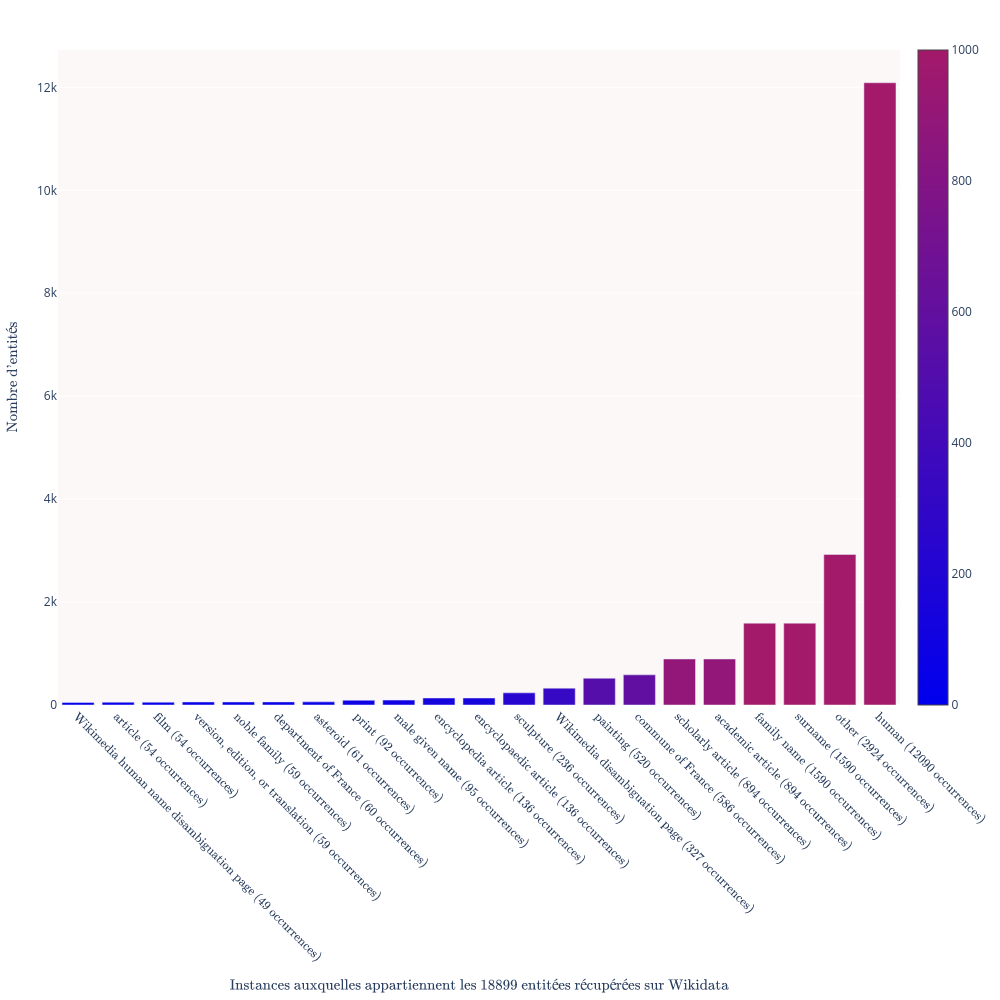
\includegraphics[width=\linewidth]{annexes/fig_wikidata_instances.png}
	\caption \\Occurrences des différentes catégories auxquelles appartiennent les entités \wkd{} liées avec les entrées de catalogues
	\label{appendix:wikidata_instances}
\end{figure}

\begin{figure}
	\centering
	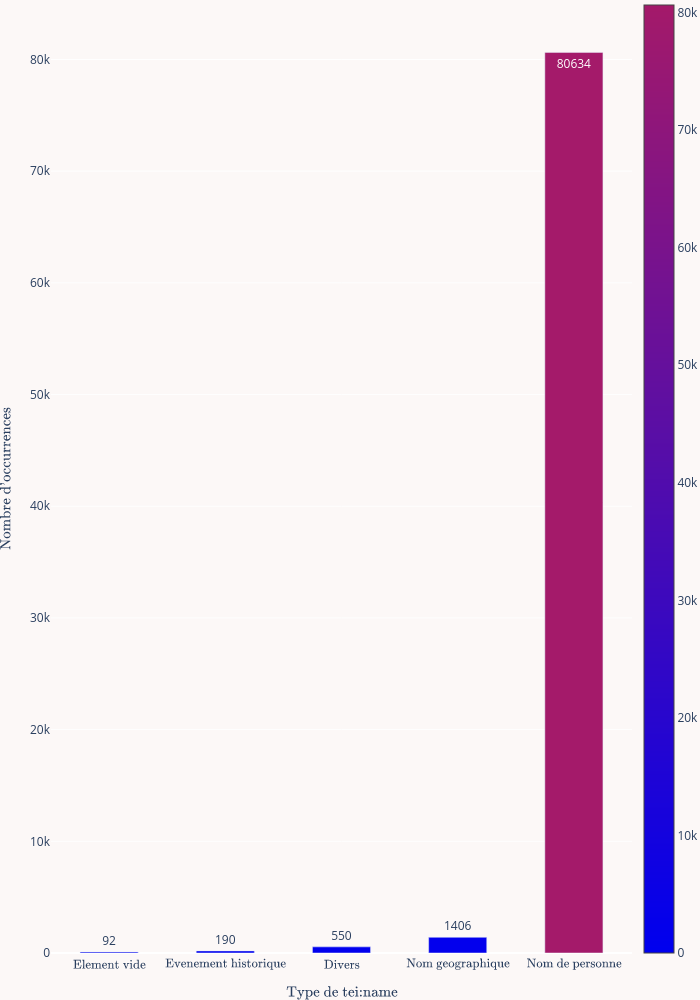
\includegraphics[width=\linewidth]{annexes/fig_teinametypes.png}
	\caption{Répartition des différents types de \tname{}}
	\label{appendix:tnametypes}
\end{figure}

\chapter{Code source et données encodées}
\begin{listing}[p]
	\begin{minted}{python}
functions = {
	"général": "general",
	"maréchal": "marshal",
	"lieutenant": "military",
	"officier": "military",
	"colonel": "military",
	"lieutenant-colonel": "military",
	"commandant": "military",
	"capitaine": "military",  # "less important" military positions
	"roi": "king",
	"empereur": "emperor",
	"president": "president",
	"homme politique": "politician",
	"président de l'assemblée": "politician",
	"orateur": "politician",
	"député": "politician",
	"secrétaire d'état": "politician",
	"sénateur": "politician",
	"écrivain": "writer",
	"auteur": "writer",
	"romancier": "writer",
	"acteur": "actor",
	"actrice": "actress",
	"cantatrice": "singer",
	"chanteur": "singer",
	"chanteuse": "singer",
	"peintre": "painter",
	"sculpteur": "sculptor",
	"statutaire": "sculptor",
	"compositeur": "composer",
	"musicien": "musician",
	"musicienne": "musician",
	"tragédien": "actor",
	"chansonnier": "chansonnier",
	"achitecte": "architect",
	"journaliste": "journalist",
	"inventeur": "inventor",
	"chimiste": "chemist",
	"connétable": "constable",
	"archevêque": "archbishop",
	"évêque": "bishop",
	"docteur": "physicist",
	"médecin": "physicist"
}		
	\end{minted}
	\caption{Table de conversion associant un métier à son équivalent normalisé}
	\label{appendix:convfunction}
\end{listing}

\clearpage
\begin{multipageminted}
	\begin{minted}{python}
dpts = [
	"ain",
	"aisne",
	"allier",
	"basses-alpes",
	"hautes-alpes",
	"alpes-maritimes",
	"annepins",
	"provence",
	"ardèche",
	"ardennes",
	"arriège",
	"arno",
	"aube",
	"aude",
	"aveyron",
	"bouches-de-l'elbe",
	"bouches-de-l'escaut",
	"bouches-de-l'yssel",
	"bpuches-de-la-meuse",
	"bouches-du-rhin",
	"bouches-du-rhône",
	"bouches-du-weser",
	"calvados",
	"cantal",
	"charente",
	"charente-inférieure",
	"cher",
	"corrèze",
	"corse",
	"côte-d'or",
	"côtes-du-nord",
	"creuse",
	"deux-nèthes",
	"deux-sèvres",
	"doire",
	"dordogne",
	"doubs",
	"drôme",
	"dyle",
	"ems-occidental",
	"ems-oriental",
	"ems-supérieur",
	"escaut",
	"eure",
	"eure-et-loir",
	"finistère",
	"forêts",
	"gard",
	"haute-garonne",
	"gers",
	"gironde",
	"hérault",
	"ille-et-villaine",
	"indre",
	"indre-et-loire",
	"isère",
	"jemappes",
	"jura",
	"landes",
	"léman",
	"loire",
	"loir-et-cher",
	"haute-loire",
	"loire-inférieure",
	"loiret",
	"lot",
	"lot-et-garonne",
	"lozère",
	"lys",
	"maine-et-loire",
	"manche",
	"marengo",
	"marne",
	"haute-marne",
	"méditerrannée",
	"mayenne",
	"meurthe",
	"meuse",
	"meuse-inférieure",
	"mont-blanc",
	"mont-tonnerre",
	"montenotte",
	"morbihan",
	"meuse",
	"moselle",
	"nièvre",
	"nord",
	"oise",
	"ombrone",
	"orne",
	"ourte",
	"paris",
	"pas-de-calais",
	"pô",
	"puy-de-dôme",
	"hautes-pyrénées",
	"basses-pyrénées",
	"pyrénées-orientales",
	"haut-rhin",
	"bas-rhin",
	"rhin-et-moselle",
	"rhône",
	"rhône-et-loire",
	"roer",
	"rome",
	"haute-saône",
	"saône-et-loire",
	"sambre-et-meuse",
	"sarre",
	"sarthe",
	"seine",
	"seine-et-marne",
	"seine-et-oise",
	"seine-inférieure",
	"sézia",
	"simplon",
	"deux-sèvres",
	"somme",
	"stura",
	"tarn",
	"tarn-et-garonne",
	"taro",
	"trasimène",
	"var",
	"vaucluse",
	"vendée",
	"vienne",
	"haute-vienne",
	"vosges",
	"yonne",
	"yssel-supérieur",
	"zuyderzée"
]		
	\end{minted}
	\caption{Liste de départements du XIXe~s. pour détecter des informations géographiques}
	\label{appendix:convdpt}
\end{multipageminted}
\clearpage

\begin{listing}[p]
	\begin{minted}{python}
countries = {
	"états-unis d'amérique": "united states of america",
	"etats-unis d'amérique": "united states of america",
	"états unis d'amérique": "united states of america",
	"etats unis d'amerique": "united states of america",
	"états-unis": "united states of america",
	"etats-unis": "united states of america",
	"etats unis": "united states of america",
	"états unis": "united states of america",
	"italie": "italy",
	"grèce": "greece",
	"canada": "canada",
	"chine": "china",
	"haïti": "haiti",
	"tobago": "tobago",
	"brésil": "brasil",
	"burkina-faso": "burkina-faso",
	"cameroun": "cameroun",
	"tchad": "tchad",
	"congo": "congo",
	"gabon": "gabon",
	"guinée": "guinea",
	"côte d'ivoire": "ivory coast",
	"mali": "mali",
	"mauritanie": "mauritania",
	"niger": "niger",
	"sénégal": "senegal",
	"madagascar": "madagascar",
	"seychelles": "seychelles",
	"tanzanie": "tanzania",
	"zanzibar": "zanzibar",
	"liban": "lebanon",
	"syrie": "syria",
	"inde": "india",
	"laos": "laos",
	"viet-nâm": "vietnam"
}	
	\end{minted}
	\caption{Table de conversion pour les pays}
	\label{appendix:convcountry}
\end{listing}

\clearpage
\begin{multipageminted}
	\begin{minted}{python}
colonies = [
	"québec",
	"ontario",
	"saint-pierre-et-miquelon",
	"mississippi",
	"missouri",
	"louisiane",
	"anguilla",
	"antigua",
	"dominique",
	"saint-domingue",
	"guadeloupe",
	"monsterrat",
	"saint-martin",
	"saint-barthélémy",
	"sainte-lucy",
	"saint-vincent-et-les-grenadines",
	"saint-eustache",
	"saint-christophe",
	"martinique"
	"guyane française",
	"guyane",
	"maroc",  # unfortunately the morocco referred to in XIXth century france is a french protectorate
	"algérie",  # same
	"algérie française",  # same
	"tunisie",  # same
	"fezzan",
	"dahomey",
	"haute-volta",
	"oubangui-chari",
	"congo français",
	"moyen-congo",
	"guinée française",
	"soudan français",
	"gorée",
	"tigi",
	"djibouti",
	"cheikh saïd",
	"comores",
	"fort-dauphin",
	"îles maurice",
	"mayotte",
	"la réunion",
	"îles éparses",
	"île amsterdam",
	"île saint-paul",
	"archipel crozet",
	"îles kerguelen",
	"castellorizo",
	"grand-liban",
	"sandjak d'alexandrette",
	"indes françaises",
	"pondichéry",
	"karikal",
	"yanaon",
	"mahé",
	"chanderngor",
	"tonkin",
	"annam",
	"cochinchine",
	"guangzhou wan",
	"shanghai",
	"guangzhou",
	"tianjin",
	"hankou",
	"clipperton",
	"nouvelle-calédonie",
	"polynésie française",
	"vanuatu",
	"nouvelles-hébrides",
	"wallis et futuna"
]
	\end{minted}
	\caption{Liste d'anciennes colonies françaises utilisées pour la détection de motifs}
	\label{appendix:convcolonie}
\end{multipageminted}
\clearpage

\begin{listing}[p]
	\begin{minted}{python}
provinces = [
	"armagnac",
	"île-de-france",
	"berry",
	"orléanais",
	"normandie",
	"languedoc",
	"lyonnais",
	"dauphiné",
	"champagne",
	"aunis",
	"saintonge",
	"poitou",
	"guyenne et gascogne",
	"bourgogne",
	"picardie",
	"anjou",
	"provence",
	"angoumois",
	"bourbonnais",
	"marche",
	"bretagne",
	"maine",
	"touraine",
	"limousin",
	"comté de foix",
	"auvergne",
	"béarn",
	"alsace",
	"artois",
	"roussillon",
	"flandre française et hainaut français",
	"franche-comté",
	"lorraine et trois-évêchés",
	"corse",
	"nivernais",
]
	\end{minted}
	\caption{Liste d'anciennes provinces françaises pour la détection de motifs}
	\label{appendix:convprov}
\end{listing}

\begin{listing}[p]
	\begin{minted}{python}
events = {
	"défense nationale": "government of national defense",
	"defense nationale": "government of national defense",
	"révolution française": "french revolution",
	"revolution francaise": "french revolution",
	"guerre de trente ans": "thirty years' war 1618 1648",
	"guerre de cent ans": "hundred years' war 1337 1453",
	"guerre de sept ans": "seven years war 1756 1763",
	"guerre": "war",
	"insurrection": "war",
	"siège de mayence": "siege of mainz",
	"siège": "siege",
	"commune": "commune",
	"défense": "battle",
	"révolution": "revolution"
}
	\end{minted}
	\caption{Table de conversion pour les évènements historiques}
	\label{appendix:convevt}
\end{listing}

\begin{listing}[p]
	\begin{minted}{python}
status = {
	"empereur": "",
	"impératrice": "",
	"géneral": "general",
	"reine": "queen",
	"roi": "king",
	"princesse": "princess",
	"prince": "prince",
	"archiduchesse": "",
	"archiduc": "",
	"duchesse": "duchess",
	"duc": "duke",
	"famille": "family",
	"seigneur": "",
	"vicomtesse": "",
	"victesse": "",
	"vicomte": "",
	"victe": "",
	"comtesse palatine": "countess palatine",
	"comtesse": "",
	"ctesse": "",
	"comte": "",
	"cte": "",
	"cardinal": "",
	"pape": "pope",
	"lord": "",
	"chevalier": "",
	"marquise": "",
	"marquis": "",
	"sire": "",
	"baronnesse": "",
	"baronne": "",
	"baron": "",
	"abbé": "",
	"madame": "",
	"mme": "",
	"monsieur": "",
	"mr": "",
	"docteur": "",
	"maréchale": "",
	"maréchal": "",
	"mademoiselle": "",
	"melle": "",
	"mlle": "",
	"sir": ""
}
	\end{minted}
	\caption{Liste de colonies pour la détection de motifs}
	\label{appendix:convstatus}
\end{listing}

\begin{listing}[p]
	\begin{minted}{python}
comp_names = {
	"arm ch": "armand-charles",
	"ch m": "charles-marie",
	"ch l f": "charles-louis-françois",
	"f m": "francois-marie",
	"fr emm.": "françois-emmanuel",
	"j ant": "jean-antoine",
	"j f": "jean-francois",
	"j m": "jean-marie",
	"j j": "jean-jacques",
	"j l": "jean-louis",
	"j b": "jean-baptiste",
	"j p": "jean-pierre",
	"j pierre": "jean-pierre",
	"l f": "louis-françois",
	"m f": "marius-felix",
	"franc rené": "francois-rené",
	"m madeleine": "marie-madeleine",
	"ph h": "philippe henri",
	"p aug": "pierre auguste",
	"p alex": "pierre alexandre",
	"p j": "pierre-jean",
	"j sylvain": "jean-sylvain",
	"l ph": "louis-philippe",
	"edm ch": "edmond-charles",
	"ch marie": "charles-marie"
}
	\end{minted}
	\caption{Table de conversion permettant de remplacer un nom abrégé composé par sa version complète}
	\label{appendix:namecomp}
\end{listing}

\begin{listing}[p]
	\begin{minted}{python}
names = {
	"ad": "adam",
	"alex": "alexandre",
	"alph": "alphonse",
	"ant": "antoine",
	"arm": "armand",
	"aug": "auguste",
	"ch": "charles",
	"cl": "claude",
	"dom": "dominique",
	"emm": "emmanuel",
	"ed": "edouard",
	"et": "etienne",
	"ét": "etienne",
	"ferd": "ferdinand",
	"fred": "frederic",
	"fr": "françois",
	"franc": "françois",
	"franç": "françois",
	"fréd": "frédéric",
	"g": "guillaume",
	"guill": "guillaume",
	"gab": "gabriel",
	"jh": "joseph",
	"jacq": "jacques",
	"jos": "joseph",
	"math": "matthieu",
	"nic": "nicolas",
	"ph": "philippe",
	"v": "victor",
	"vr": "victor",
}
	\end{minted}
	\caption{Table de conversion permettant de remplacer un nom abrégé non composé par sa version complète}
	\label{appendix:namesimp}
\end{listing}

\clearpage
\begin{multipageminted}
	\begin{minted}[breakanywhere]{python}
def rgx_abvcomp(nstr):
	"""
	try to extract an abbreviated composed first name. if there is no match, return None
	pattern
	-------
	the patterns in the example below are simplified to keep things readable
	- two strings separated by a "-" or "\s"
	- the first or second string can be a full name ([A-Z][a-z]+)
	or an abbreviation ([A-Z][a-z]*\.)
	- if the strings are separated by "\s", they must be finished by "\."
	(to be sure that we don't capture full names, i.e: "J. Ch."  can be captured,
	but not "Jean Charles")
	- complex names with 3 or more words must have "-" and at least one "\."
	- (\s|$) and (^|\s) are safeguards to avoid matching the end or beginning of another word
	examples
	--------
	matched : M.-Madeleine Pioche de la Vergne  # matched string : M.-Madeleine
	matched : C.-A. de Ferriol  # matched string : C.-A.
	matched : J. F.  # matched string : J. F.
	matched : Jean F.  # matched string : Jean F.
	matched : Jean-F.  # matched string : Jean-F.
	matched : A M  # matched string : A M
	matched : C.-Edm.-G.  # matched string : C.-Edm.-G.
	matched : Charles-Edm.-G.  # matched string : Charles-Edm.-G.
	not matched : Anne M
	not matched : Claude Henri blabla
	not matched : Claude Henri
	:param nstr: the name string used as input
	:return: the matched string if there is a match ; None if there is no match
	"""
	mo = re.search(r"(^|,|\s)[A-ZÀÂÄÈÉÊËÏÔŒÙÛÜŸ][a-zàáâäéèêëíìîïòóôöúùûüøœæç]*"
			+ "\.?-[A-ZÀÂÄÈÉÊËÏÔŒÙÛÜŸ][a-zàáâäéèêëíìîïòóôöúùûüøœæç]*\.(\s|,|$)", nstr) \
		 or re.search(r"(^|,|\s)[A-ZÀÂÄÈÉÊËÏÔŒÙÛÜŸ][a-zàáâäéèêëíìîïòóôöúùûüøœæç]*\."
			+ "-[A-ZÀÂÄÈÉÊËÏÔŒÙÛÜŸ][a-zàáâäéèêëíìîïòóôöúùûüøœæç]*\.?(\s|,|$)", nstr) \
		 or re.search(r"(^|,|\s)[A-ZÀÂÄÈÉÊËÏÔŒÙÛÜŸ]\.?\s"
			+ "[A-ZÀÂÄÈÉÊËÏÔŒÙÛÜŸ][a-zàáâäéèêëíìîïòóôöúùûüøœæç]*\.(\s|,|$)", nstr) \
		 or re.search(r"(^|,|\s)[A-ZÀÂÄÈÉÊËÏÔŒÙÛÜŸ][a-zàáâäéèêëíìîïòóôöúùûüøœæç]*\.?"
		    + "\s[A-ZÀÂÄÈÉÊËÏÔŒÙÛÜŸ]\.(\s|,|$)", nstr) \
		 or re.search(r"(^|,|\s)[A-ZÀÂÄÈÉÊËÏÔŒÙÛÜŸ]\.?\s[A-ZÀÂÄÈÉÊËÏÔŒÙÛÜŸ]\.?(\s|,|$)", nstr) \
		 or re.search(r"([A-ZÀÂÄÈÉÊËÏÔŒÙÛÜŸ]\.){2,}", nstr) \
		 or re.search(r"(^|,|\s)([A-ZÀÂÄÈÉÊËÏÔŒÙÛÜŸ][a-zàáâäéèêëíìîïòóôöúùûüøœæç]*\.?-)+"
			+ "([A-ZÀÂÄÈÉÊËÏÔŒÙÛÜŸ][a-zàáâäéèêëíìîïòóôöúùûüøœæç]*\.)(\s|,|$)", nstr) \
		 or re.search(r"(^|,|\s)([A-ZÀÂÄÈÉÊËÏÔŒÙÛÜŸ][a-zàáâäéèêëíìîïòóôöúùûüøœæç]*\.-)+"
		  	+ "([A-ZÀÂÄÈÉÊËÏÔŒÙÛÜŸ][a-zàáâäéèêëíìîïòóôöúùûüøœæç]*\.?)(\s|,|$)", nstr)
	if mo is not None:
		return mo[0]
	else:
		return None
	\end{minted}
	\caption{Fonction permettant d'identifier et d'extraire un nom abrégé composé}
	\label{appendix:rgxabvcomp}
\end{multipageminted}
\clearpage

\begin{listing}[p]
	\begin{minted}[breakanywhere]{python}
def rgx_abvsimp(nstr):
	"""
	try to extract a "simple" (not composed) abbreviated first name. if there is no match, return None
	pattern
	-------
	a capital letter (possibly followed by a certain number of lowercase letters)
	ended with a dot. (\s|$) and (^|\s) are safeguards to avoid matching the beginning
	end of another word.
	*warning* : it can also capture parts of composed abbreviated names => must be used
	in an if-elif after trying to match a composed abbreviated name
	examples
	--------
	matched : bonjour Ad.  # matched string : Ad.
	matched : J. baronne  # matched string : J.
	matched : J. F.  # matched string : J.
	matched : Jean F.  # matched string : F.
	not matched : A.-M.
	not matched : Anne M
	not matched : Hector
	:param nstr: the name string used as input
	:return:
	"""
	mo = re.search(r"(^|\s)[A-ZÀÂÄÈÉÊËÏÔŒÙÛÜŸ][a-zàáâäéèêëíìîïòóôöúùûüøœæç]*\.(\s|$|,)", nstr)
	if mo is not None:
		return mo[0]
	else:
		return None
	\end{minted}
	\caption{Fonction permettant de repérer et d'extraire un nom abrégé simple}
	\label{appendix:rgxabvsimp}
\end{listing}

\begin{listing}[p]
	\begin{minted}[breakanywhere]{python}
def rgx_complnm(nstr):
	"""
	try to extract a complete name from a string. if there is noœ match, return None
	pattern
	-------
	- an uppercase letter followed by several lowercase letters ;
	- this pattern can be repeated several times, separated by a space or "-"
	- (\s|$) and (^|\s) are safeguards to avoid matching the beginning or end of another word.
	:param nstr: the string from which a name should be extracted
	:return:
	"""
	mo = re.search(r"(^|\s)[A-ZÀÂÄÈÉÊËÏÔŒÙÛÜŸ][a-zàáâäéèêëíìîïòóôöúùûüøœæç]+"
		+ "((\s|-)[A-ZÀÂÄÈÉÊËÏÔŒÙÛÜŸ][a-zàáâäéèêëíìîïòóôöúùûüøœæç]+)*($|\s|,)", nstr)
	if mo is not None:
		return mo[0]
	else:
		return None
	\end{minted}
	\caption{Fonction permettant d'identifier et d'extraire un nom complet non abrégé}
	\label{appendix:rgxfull}
\end{listing}
\pagebreak

\clearpage
\begin{figure}[!htb]
	\begin{subfigure}{\textwidth}
		\begin{minted}{xml}
<item n="264" xml:id="CAT_000327_e264">
	<!-- ... -->
	<name type="author">Spontini (Gaspard)</name>
	<trait>
		<p>célèbre compositeur, auteur de la Vestale, né en 1779, mort en 1851.</p>
	</trait>
	<!-- ... -->
</item>
		\end{minted}
		\subcaption{La source \xmltei{}}
	\end{subfigure}
	\begin{subfigure}{\textwidth}
		\begin{minted}{python}
{
	'fname': 'gaspard ', 
	'lname': 'spontini ', 
	'nobname_sts': '', 
	'status': '', 
	'dates': '1779 1851 ', 
	'function': 'writer', 
	'rebuilt': False
}
		\end{minted}
		\caption{Le dictionnaire d'informations structurées}
	\end{subfigure}
	\begin{subfigure}{\textwidth}
		\begin{lstlisting}
gaspard spontini 1779 1851 writer
gaspard spontini 1851 writer
gaspard spontini 1779 writer
gaspard spontini writer
spontini 1779 1851 writer
spontini 1851 writer
spontini 1779 writer
spontini writer
		\end{lstlisting}
		\caption{Les recherches lancées sur l'\api{} \wkd{}}
	\end{subfigure}
	\caption{De la \tei{} à l'\api{}: document en entrée, informations extraites et chaînes de caractères recherchées}
	\label{code:apipipeline}
\end{figure}
Ci dessus (\ref{code:apipipeline}) sont présentés l'entrée et les données produites lors de l'alignement avec \wkd{}: en premier les données en entrée, ensuite les informations qui en sont extraites et enfin les différentes chaînes de caractères recherchées. Il est à noter que, dans la plupart des cas, seules une ou deux recherches sont faites sur l'\api{} avant d'obtenir un résultat; ici, huit chaînes différentes ont été construites et recherchées, ce qui représente l'intégralité de l'algorithme.
\clearpage

\begin{multipageminted}
	\inputminted[breakanywhere]{python}{./annexes/sparql_result.json}
	\caption{Exemple de réponse \sparql{} au format \json{} pour la requête \ref{code:sparql}}
	\label{appendix:sparqlout_json}
\end{multipageminted}
\clearpage

\begin{multipageminted}
	\inputminted[breakanywhere]{xml}{./annexes/sparql_result.xml}
	\caption{Exemple de réponse \sparql{} au format \xml{} pour la requête \ref{code:sparql}}
	\label{appendix:sparqlout_xml}
\end{multipageminted}
\clearpage

\begin{multipageminted}
	\begin{minted}[breakanywhere]{python}
{
	# entrées précédentes...
	"Q108438226": {
		"instance": [
			"Q3305213"
		],
		"instanceL": [
			"painting"
		],
		"gender": [],
		"genderL": [],
		"citizenship": [],
		"citizenshipL": [],
		"lang": [],
		"langL": [],
		"deathmanner": [],
		"deathmannerL": [],
		"birthplace": [],
		"birthplaceL": [],
		"deathplace": [],
		"deathplaceL": [],
		"residplace": [],
		"residplaceL": [],
		"burialplace": [],
		"burialplaceL": [],
		"educ": [],
		"educL": [],
		"religion": [],
		"religionL": [],
		"occupation": [],
		"occupationL": [],
		"award": [],
		"awardL": [],
		"position": [],
		"positionL": [],
		"member": [],
		"memberL": [],
		"nobility": [],
		"nobilityL": [],
		"workcount": [],
		"conflictcount": [],
		"img": [
			"http://commons.wikimedia.org/wiki/Special:FilePath/Louis%20de%20Frott%C3%A9.jpg"
		],
		"signature": [],
		"birth": [],
		"death": [],
		"title": [
			"Louis de Frott\u00e9 (1755-1800), g\u00e9n\u00e9ral vend\u00e9en"
		],
		"inception": [
			"1822-01-01"
		],
		"author": [],
		"authorL": [],
		"pub": [],
		"pubL": [],
		"pubplace": [],
		"pubplaceL": [],
		"pubdate": [],
		"creator": [
			"Q51077254"
		],
		"creatorL": [
			"Louise Bouteiller"
		],
		"material": [
			"Q12321255",
			"Q296955"
		],
		"materialL": [
		"canvas",
			"oil paint"
		],
		"height": [
			"216"
		],
		"genre": [
			"Q134307"
		],
		"genreL": [
			"portrait"
		],
		"movement": [],
		"movementL": [],
		"creaplace": [],
		"creaplaceL": [],
		"viafID": [],
		"bnfID": [],
		"isniID": [],
		"congressID": [],
		"idrefID": []
	},
	"Q3383960": {
		"instance": [
			"Q5"
		],
		"instanceL": [
			"human"
		],
		"gender": [
			"Q6581097"
		],
		"genderL": [
			"male"
		],
		"citizenship": [
			"Q142"
		],
		"citizenshipL": [
			"France"
		],
		"lang": [
			"Q150"
		],
		"langL": [
			"French"
		],
		"deathmanner": [],
		"deathmannerL": [],
		"birthplace": [
			"Q1148468"
		],
		"birthplaceL": [
			"Vendargues"
		],
		"deathplace": [],
		"deathplaceL": [],
		"residplace": [],
		"residplaceL": [],
		"burialplace": [],
		"burialplaceL": [],
		"educ": [],
		"educL": [],
		"religion": [],
		"religionL": [],
		"occupation": [
			"Q47064",
			"Q82955",
			"Q189290"
		],
		"occupationL": [
			"military personnel",
			"politician",
			"military officer",
			"officer"
		],
		"award": [
			"Q10855226",
			"Q11593374",
			"Q1313340"
		],
		"awardL": [
			"Grand Croix of the L\u00e9gion d'honneur",
			"Knight of the Royal and Military Order of Saint Louis",
			"names inscribed under the Arc de Triomphe",
			"Grand Cross of the Legion of Honour"
		],
		"position": [
			"Q21032625",
			"Q15904689"
		],
		"positionL": [
			"member of the Chamber of Peers",
			"Governor of Algeria"
		],
		"member": [],
		"memberL": [],
		"nobility": [
			"Q165503"
		],
		"nobilityL": [
			"baron"
		],
		"workcount": [],
		"conflictcount": [
			"1"
		],
		"img": [
			"http://commons.wikimedia.org/wiki/Special:FilePath/Berthez%C3%A8ne.JPG"
		],
		"signature": [],
		"birth": [
			"1775-03-24"
		],
		"death": [
			"1847-10-09"
		],
		"title": [],
		"inception": [],
		"author": [],
		"authorL": [],
		"pub": [],
		"pubL": [],
		"pubplace": [],
		"pubplaceL": [],
		"pubdate": [],
		"creator": [],
		"creatorL": [],
		"material": [],
		"materialL": [],
		"height": [],
		"genre": [],
		"genreL": [],
		"movement": [],
		"movementL": [],
		"creaplace": [],
		"creaplaceL": [],
		"viafID": [
			"15030322"
		],
		"bnfID": [
			"14643064j"
		],
		"isniID": [
			"0000 0000 4820 9162"
		],
		"congressID": [
			"n2005062361"
		],
		"idrefID": [
			"088623629"
		]
	},
	# entrées suivantes...
}
	\end{minted}
	\caption{Extrait de la base de connaissance constituée grâce à \sparql{} suite  à l'alignement avec des entités \wkd{}}
	\label{appendix:dbextract}
\end{multipageminted}
\clearpage

\begin{listing}[p]
	\begin{minted}{xml}
<listPrefixDef>
	<prefixDef 
		ident="wd" 
		matchPattern="(Q[0-9]+)" 
		replacementPattern="https://www.wikidata.org/wiki/$1">
		<p>
			In the <gi>body</gi>, the <att>ref</att> attributes 
			containted in <gi>name</gi> elements are pointing to to a
			<ref target="https://www.wikidata.org/wiki/">Wikidata</ref> 
			identifier by using the <code>wd:</code> prefix. This <gi>prefixDef</gi>
			allows to rebuilt the complete URL from a wikidata identifier by 
			replacing the <code>wd:</code> prefix with:
			<code>https://www.wikidata.org/wiki/</code>.
		</p>
	</prefixDef>
</listPrefixDef>
	\end{minted}
	\caption{Le \texttt{tei:listPrefixDef} décrivant le rôle du préfixe \enquote{wd} dans les catalogues}
	\label{appendix:listprefixdef}
\end{listing}
\clearpage

\begin{multipageminted}
	\inputminted[breakanywhere]{xml}{annexes/api_item.xml}
	\caption{Exemple de réponse de \textit{KatAPI} au niveau \texttt{item} en \tei{}}
	\label{appendix:api_item_xml}
\end{multipageminted}
\clearpage

\begin{multipageminted}
	\inputminted[breakanywhere]{python}{annexes/api_item.json}
	\caption{Exemple de réponse de \textit{KatAPI} au niveau \texttt{item} en \json{}}
	\label{appendix:api_item_json}
\end{multipageminted}
\clearpage

\begin{multipageminted}
	\inputminted[breakanywhere]{xml}{annexes/api_cat_stat.xml}
	\caption{Exemple de réponse de \textit{KatAPI} au niveau \texttt{cat\_stat} en \tei{}}
	\label{appendix:api_cat_stat_xml}
\end{multipageminted}
\clearpage

\begin{multipageminted}
	\inputminted[breakanywhere]{python}{annexes/api_cat_stat.json}
	\caption{Exemple de réponse de \textit{KatAPI} au niveau \texttt{cat\_stat} en \json{}}
	\label{appendix:api_cat_stat_json}
\end{multipageminted}
\clearpage

\begin{multipageminted}
	\inputminted[breakanywhere]{xml}{annexes/api_error.xml}
	\caption{Exemple de message d'erreur reçu par \textit{KatAPI} en \tei{}}
	\label{appendix:api_error_xml}
\end{multipageminted}
\clearpage

\begin{multipageminted}
	\inputminted[breakanywhere]{python}{annexes/api_error.json}
	\caption{Exemple de message d'erreur reçu par \textit{KatAPI} en \json{}}
	\label{appendix:api_error_json}
\end{multipageminted}
\clearpage


\chapter{Images}
\begin{figure}[p]
	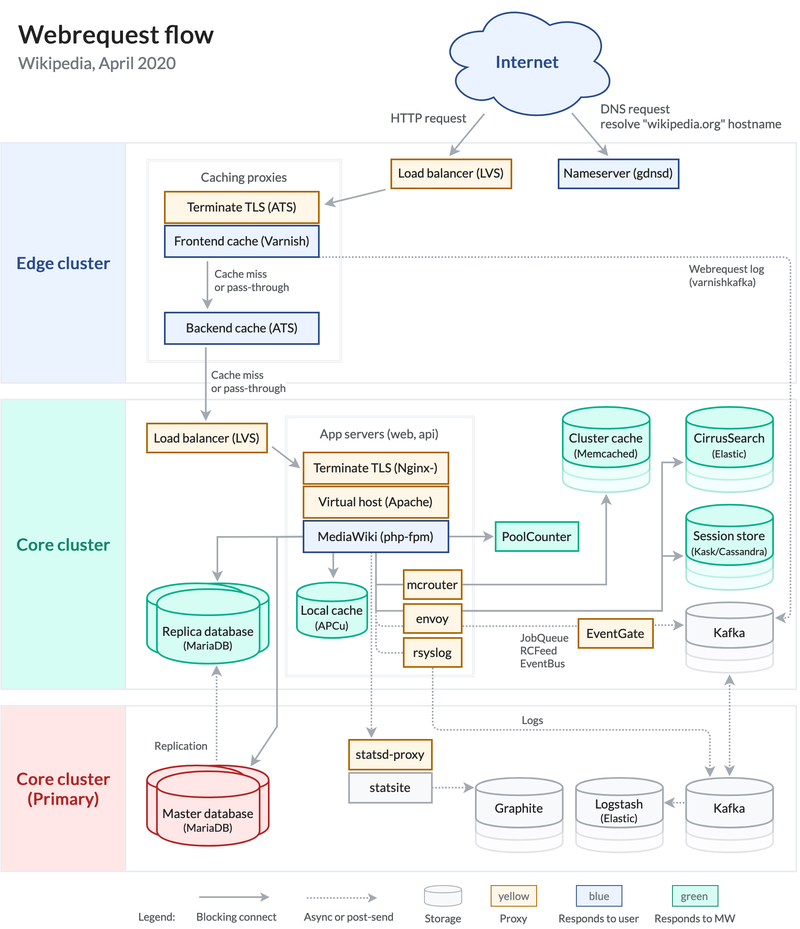
\includegraphics[width=\textwidth]{annexes/wikimedia_db_2020.png}
	\caption{L'architecture des bases de données de la \textit{Wikimedia Foundation} (schéma réalisé par Timo Tijhof en 2020, disponible dans le domaine public avec la licence Creative Commons CC0.1.0 Universal Public Domain License)}
	\label{appendix:wikimedia_db}
\end{figure}

	\begin{figure}[p]
		\centering
		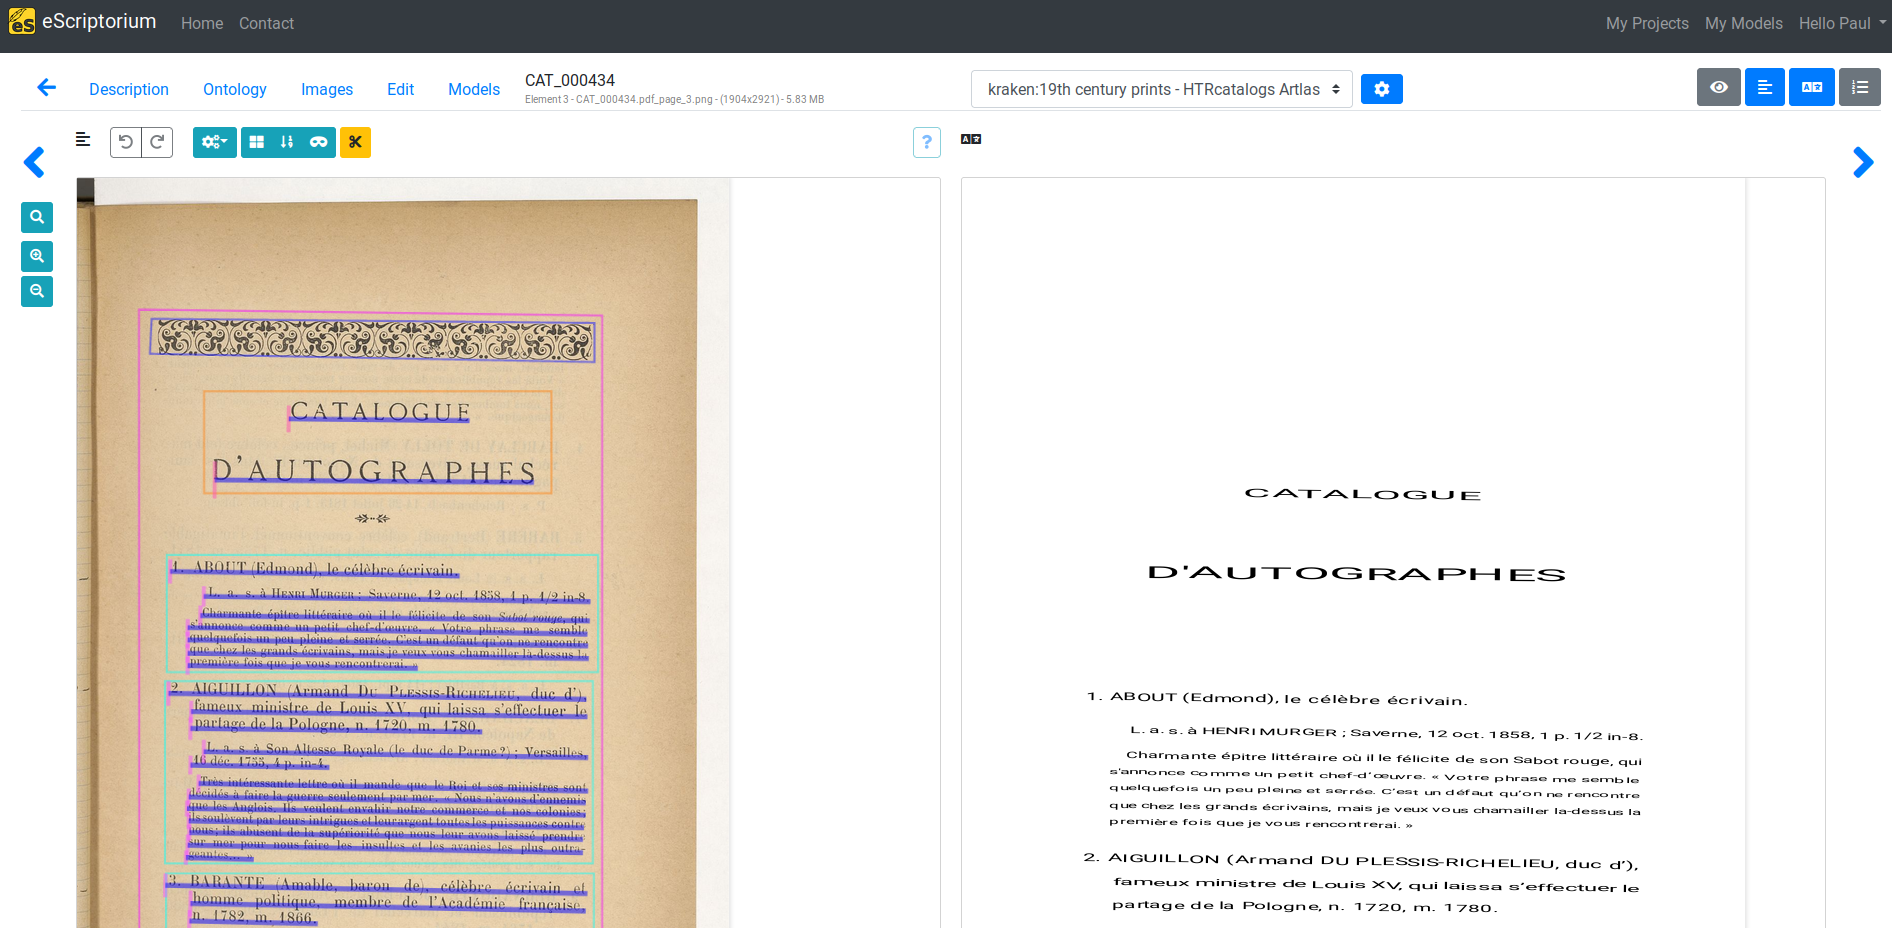
\includegraphics[width=\textheight,angle=90]{annexes/escriptorium.png}
		\caption{Capture d'écran du logiciel \textit{eScriptorium}}
		\label{appendix:escriptorium}
	\end{figure}